\section{Experiments}\label{sec:exp}


\begin{figure*}[ht!]
\centering
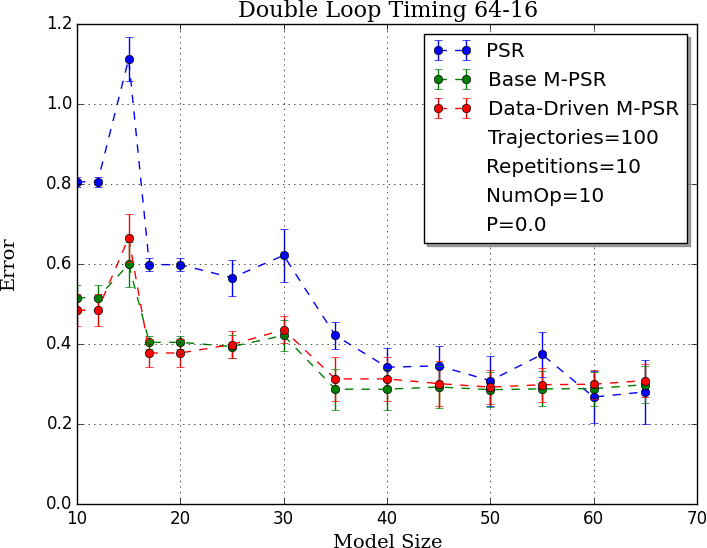
\includegraphics[width=45mm]{uCOREPICS/DL/64-16-100.png}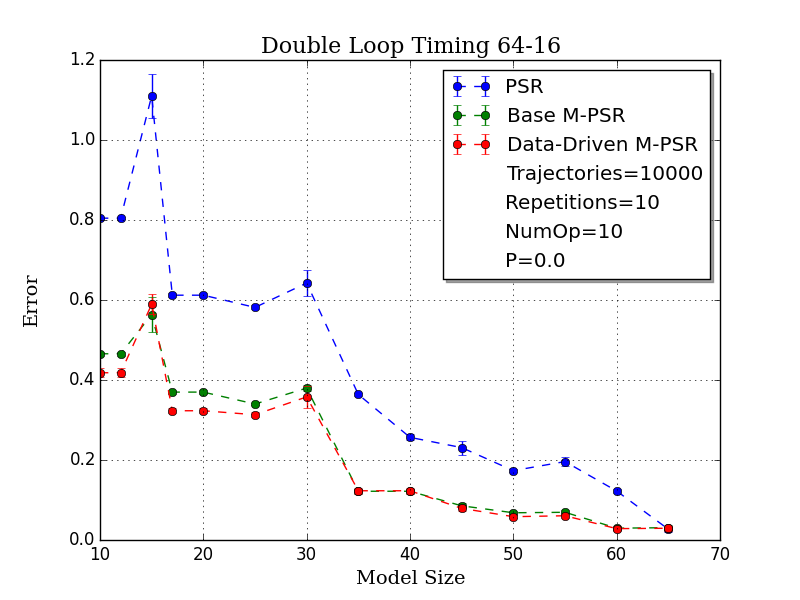
\includegraphics[width=45mm]{uCOREPICS/DL/64-16-10000.png}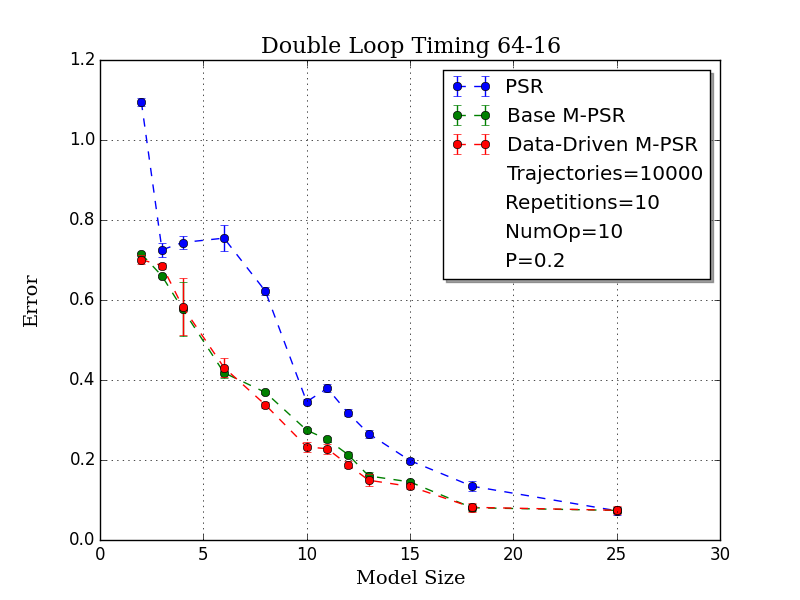
\includegraphics[width=45mm]{uCOREPICS/DL/NoiseInfo.png}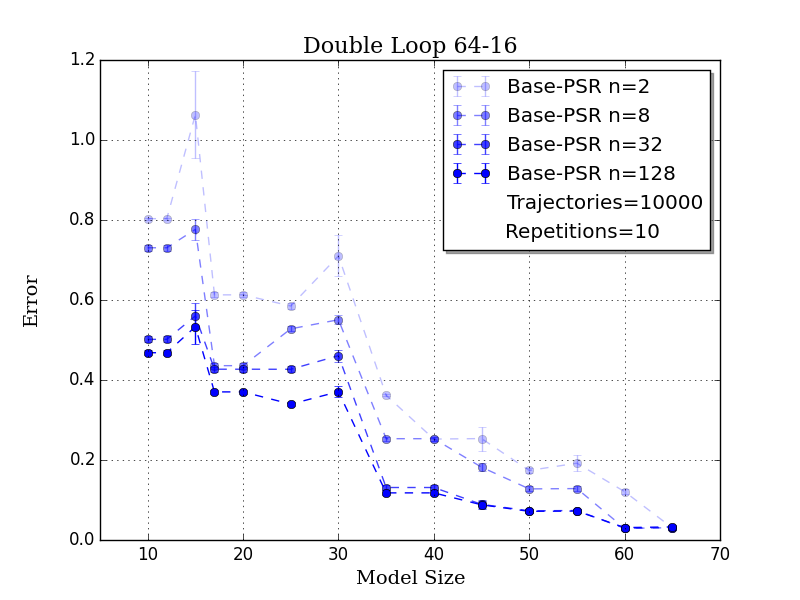
\includegraphics[width=45mm]{uCOREPICS/DL/basePows.png}

\caption{Results for the Double Loop of size 64-16 with (in order) a low amount of data, high amount of data and varying amount of noise (right two panels)\label{fig-double}}
\end{figure*}


In this section, we assess the performance of PSRs and M-PSRs in various environments, with different model sizes, and learned from both large and small datasets. For all the plots, the x-axis is model size of the PSR/M-PSRs and the y-axis is an error measurement of the learned PSR/M-PSRs.

In all the experiments, an agent is positioned in  a partially observable environment and navigates  stochastically based on state to state transition probabilities. An observation symbol is produced on every transition. When the agent exits, we record the concatenation of the symbols produced, which represents the observation sequence for the completed trajectory.  We perform experiments in two environments: a Double Loop maze and a Pacman-style environment.

For the Base M-PSR (i.e., the timing models), we construct the empirical Hankel matrix by taking $\Ps, \Ss = \{a^i, \forall i \leq n\}$, where $n$ is an application-dependent parameter. For Double Loop environments, we set $n = 150$, while for the Pacman domain, $n = 600$. For these choices of $n$, we verify that as the amount of data increases, the learned PSR with the true model size converges to the true model. For the Base M-PSR, we set $b=2, K=8$, so that the longest string in $\Sigma'$ is $a^{256}$.

For the tasks with multiple observations, a slightly more complex approach is required to choose $\Ps$ and $\Ss$. For the prefixes $\Ps$, we select the $k$ most frequent prefixes from our observation set. For the suffixes $\Ss$, we take all suffixes that occur in $\Ps$. We also require prefix completeness. That is, if $p'$ is a prefix of $p \in \Ps$, then $p' \in \Ps$. This heuristic for constructing empirical Hankel matrices was given in previous work~\cite{icml12}. For the Base M-PSR, we take $K=8$ and $B=2$ for both symbols $\Sigma=\{g,b\}$, where $g$ stands for green and $b$ for blue. For the Tree M-PSR, we set $L=7$ for a total of 128 operators, a far larger limit  than for the other M-PSRs. 

%\subsection{Measuring Performance}

To measure the performance of a PSR/M-PSR we use the following norm:
\begin{equation*}
\|f - \hat{f}\|_2 = \sqrt{\sum_{x \in \Sstar}(f(x) - \hat{f}(x))^2} \enspace,
\end{equation*}
where $f$ denotes the true probability distribution over observations and $\hat{f}$ denotes the function associated with the learned M-PSR/PSR. In our environments, $f$ can be computed exactly, as we have access to the underlying HMMs.

Since the set of observations $\Sigma^{\star}$ is infinite, we compute approximations to this error norm by fixing a set of strings $T$ and summing over it. For the Base M-PSR (timing) case, we take $T = \{a^i, \forall i \leq C\}$ with $C=600$. Importantly, $C$ has to be  large enough, such that $\sum_{i=0}^{C} f(a^i)>0.99$. For the multiple observation case, we take all possible strings that can be produced from the prefixes and suffixes in our dataset: $T = \{ps, \forall p \in \Ps, \forall s \in \Ss\} $

%\lucas{Need citation for bound on norm2 error}

\subsection{Double Loop Timing}

We start by considering the Double Loop environment, and the task of learning timing models. The length of a loop is the number of states in the loop. A trajectory begins with the agent at the intersection of the two loops. Here, the agent has a 50\% probability of entering either loop. At intermediate states, the agent moves to the next state in the loop with probability $1-P$ or remains in its current state with probability $P$. Exit states are located halfway into each loop. The agent leaves the environment at exit states with 50\% probability. 

%\subsection{Number of Trajectories}

Figure~\ref{fig-double} provides results for the case in which one loop consists of 64 states and the other of 16 states. The leftmost panel presents the results when learning from  100 observation sequences, while the results in the next panel are obtained using 10000 observations. In both cases, the M-PSRs  outperform the simple PSR for small model sizes. The right panels show the effect of 
varying the self-transition probability $P$, in order to to simulate noise in the environment. The two panels show curves of $P=0.2$ and $P=0$ respectively. We find that the environment with noisy loops is more compressible, that is, one can achieve better performance for low model sizes, but the performance becomes worse as the model size attains the environment's true size. M-PSRs still significantly outperform the standard PSR for reduced model sizes.  The rightmost panel also illustrates the effect of $K$ on the performance of the Base M-PSRs. We note that larger values of $K$ have better performance, up to $K=7$.

In Figure~\ref{fig-numops}, we illustrate how varying the number of multi-step transition operators affects performance for the 64-16 double loop. As expected, a higher number of operators improves performance, but the effect tapers off at about 20 operators. Here, the most important operators are: $\{a,a^{8},a^{24},a^{32},a^{72}\}$ which are closely tied to the environment's periodic structure.

\begin{figure}[ht!]
\centering
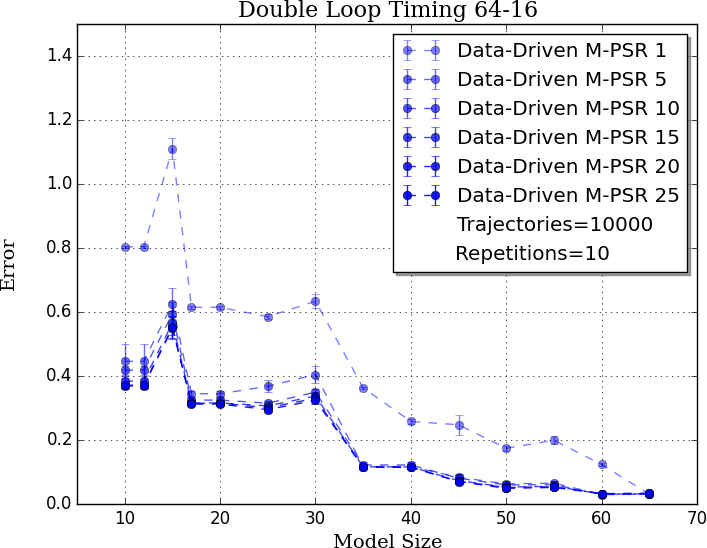
\includegraphics[width=60mm]{uCOREPICS/DL/NumOpsTiming.png}
\caption{Varying NumOps\label{fig-numops}}
\end{figure} 

\subsection{Loop Lengths}

In Figure~\ref{fig-dl47}, we plot the results of a 47-27 labyrinth.  Here, because of the lengths of the loops, observations will not be as compactly expressed from the Base M-PSR. Again, M-PSRs outperform the standard PSR for reduced model sizes.

\begin{figure}[ht!]
\centering
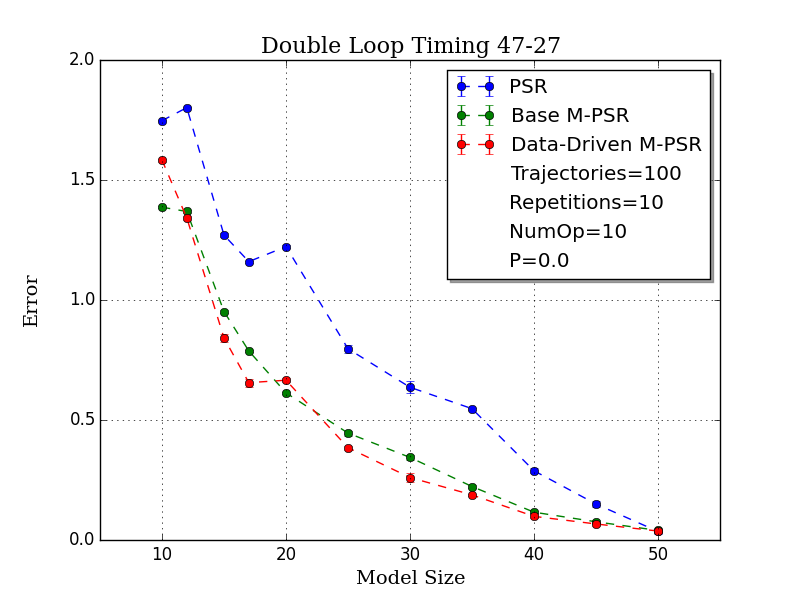
\includegraphics[width=60mm]{uCOREPICS/DL/47-27-10000.png}
\caption{High Data Double Loop 47-27\label{fig-dl47}}
\end{figure}

\subsection{Large Labyrinth Timing}

We now turn our attention to a larger labyrinth environment, similar to a Pacman game. Transitions to new states occur with equal probability. The weight $w(u,v)$ between states $u$ and $v$ corresponds to the number of time steps taken to get from $u$ to $v$. We add a parameter $sF$ (stretch factor) which is used to scale all of the weights in the graph. 


\begin{figure}[ht!]
\centering
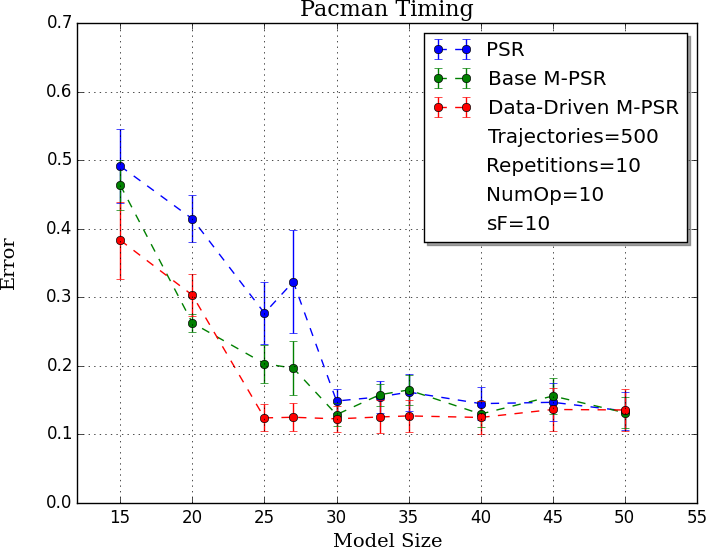
\includegraphics[width=60mm]{uCOREPICS/Pacman/Pacman500.png}
\caption{Low Data Pacman Labyrinth\label{fig-paclow}}
\end{figure}


In Figures~\ref{fig-paclow} and \ref{fig-pachigh} we vary the number of observations used for learning. M-PSRs outperform the traditional PSR regardless of the amount of data. 
\begin{figure}[ht!]
\centering
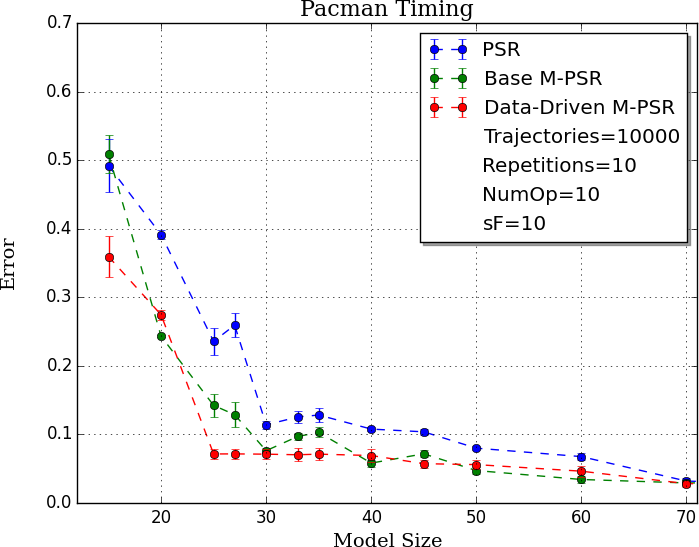
\includegraphics[width=60mm]{uCOREPICS/Pacman/Pacman10k.png}
\caption{High Data Pacman Labyrinth\label{fig-pachigh}}
\end{figure}


In Figures~\ref{fig-pachigh},\ref{fig-pacsf1} and \ref{fig-pacsf5} we vary the stretch factor parameter, while  keeping the size of the dataset fixed. We find that a higher values of sF (such as in \ref{fig-pachigh} provide increased improvement of the M-PSR relative to the standard PSR.

\begin{figure}[ht!]
\centering
\includegraphics[width=60mm]{uCOREPICS/Pacman/PacmanSF=1.png}
\caption{Stretch Factor: 1\label{fig-pacsf1}}
\end{figure}

\begin{figure}[ht!]
\centering
\includegraphics[width=60mm]{uCOREPICS/Pacman/PacmanSF=5.png}
\caption{Stretch Factor: 5\label{fig-pacsf5}}
\end{figure}

\subsection{Multiple Observations: Coloured Loops}

We now move to the multiple observation case. We construct a Double Loop environment where the first loop has length $l_1=27$ and observations are green. The second loop is blue, with length $l_2=17$. We fix the length of each trajectory at 
$3 (l_1 + l_2)$

We build empirical estimates for the Hankel matrix as follows:
\begin{equation*}
%f(x)=\dfrac{count([s \in Obs, s=x])}{count([s \in Obs, |s| \geq x])} 
f(x) = \frac{|\mathrm{train} \cap x \sstar |}{|\mathrm{train} \cap \Sigma^{\geq |x|}|} \enspace.
\end{equation*}  
This means that the PSRs will compute the probability of $x$ occurring as a prefix.


As for the timing case, we vary the amount of data used to  learn the PSRS/M-PSRs in Figures~\ref{fig-collow} and \ref{fig-colhigh}. Once again, we find M-PSRs perform far better, especially the Data-Driven M-PSR.


\begin{figure}[ht!]
\centering
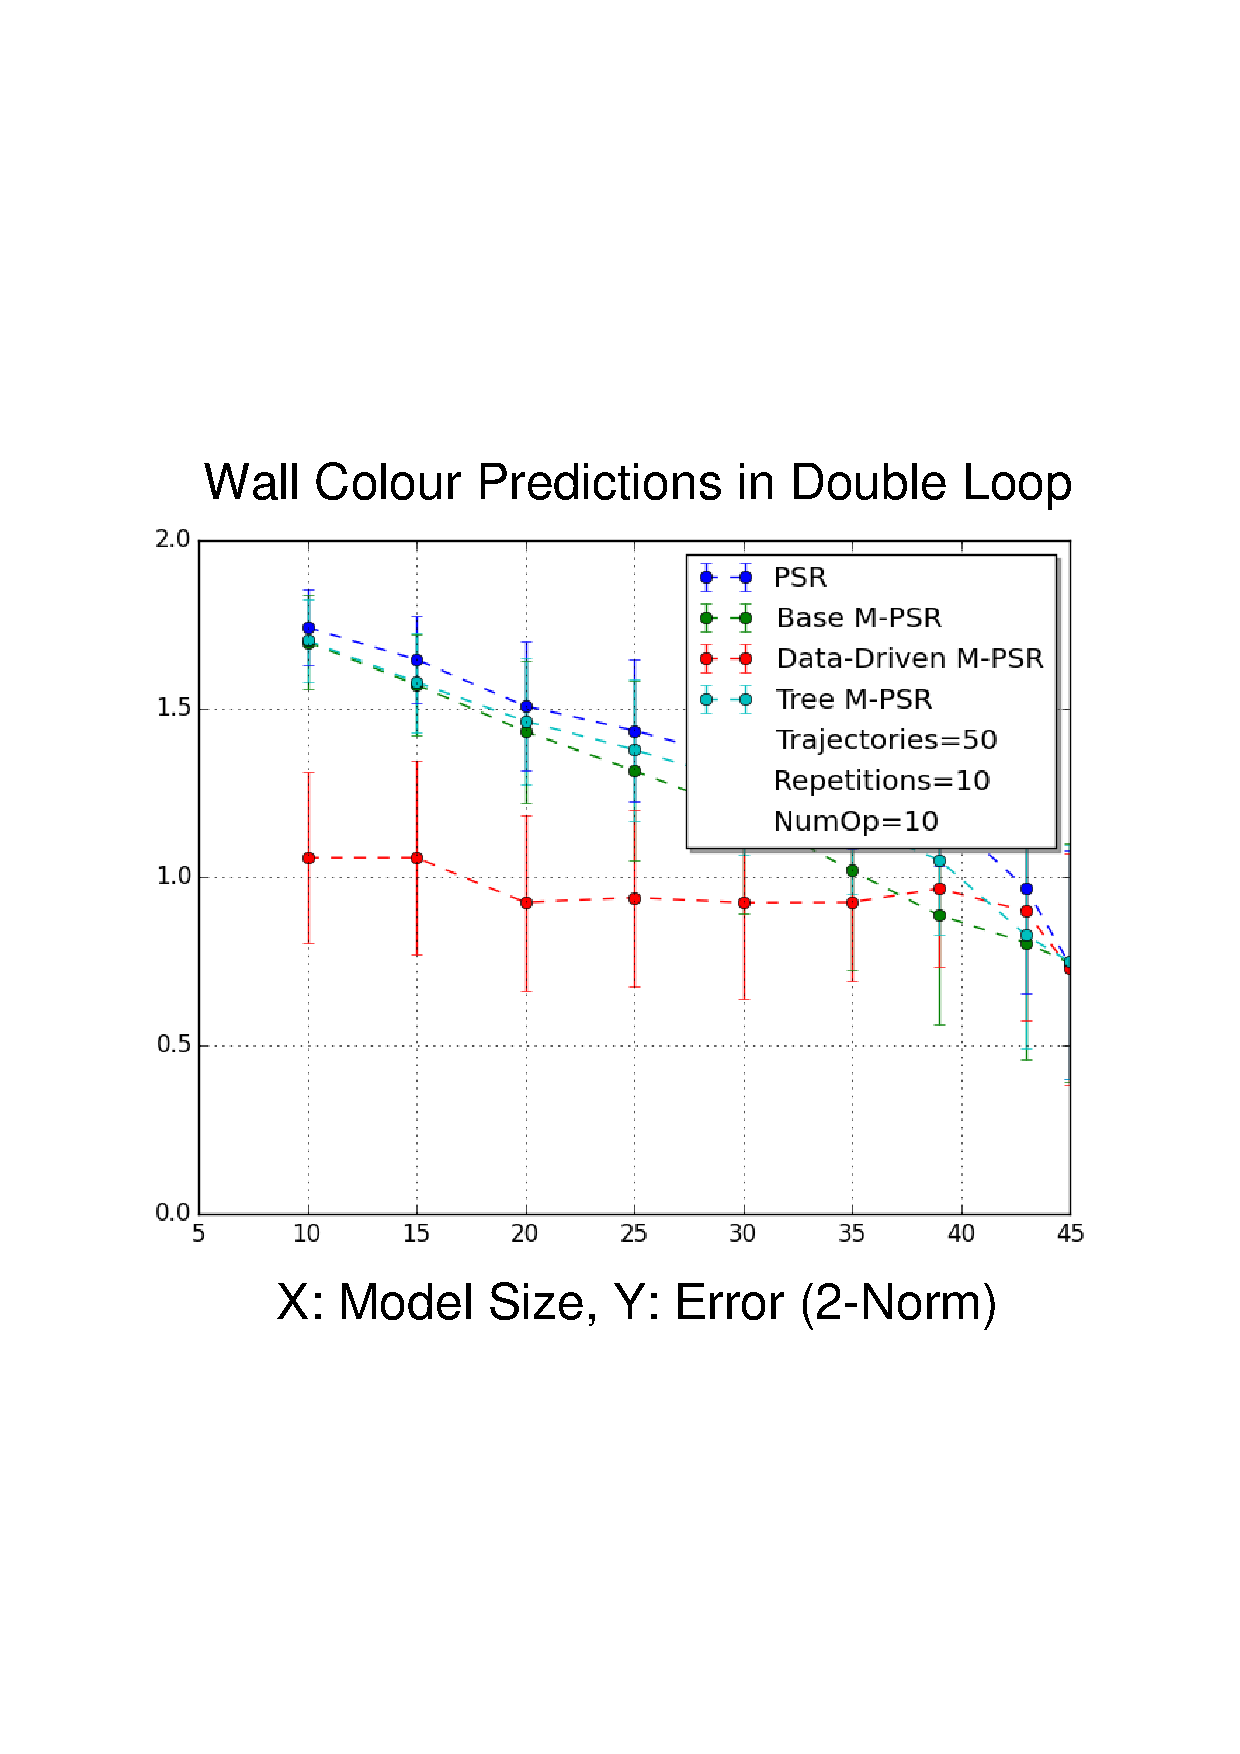
\includegraphics[width=60mm]{uCOREPICS/DLMO/MO_50.png}
\caption{Low Data Colored Loops 27-17\label{fig-collow}}
\end{figure}

\begin{figure}[ht!]
\centering
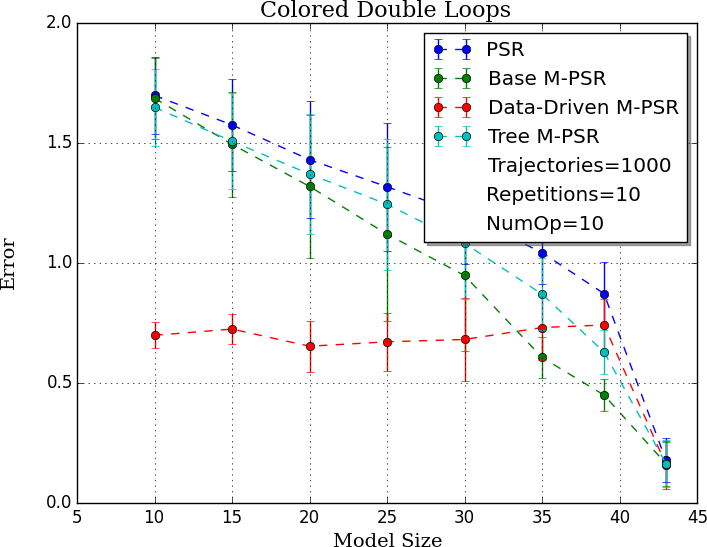
\includegraphics[width=60mm]{uCOREPICS/DLMO/MO_1k.png}
\caption{High Data Colored Loops 27-17\label{fig-colhigh}}
\end{figure}



In Figure~\ref{fig-colnumops}, we vary the number of multi-step transition operators learned. The important operators learned are $\{g,b,g^{27},b^{17}\}$, which is again very encouraging, as it reflects the structure of this particular environment.

\begin{figure}[ht!]
\centering
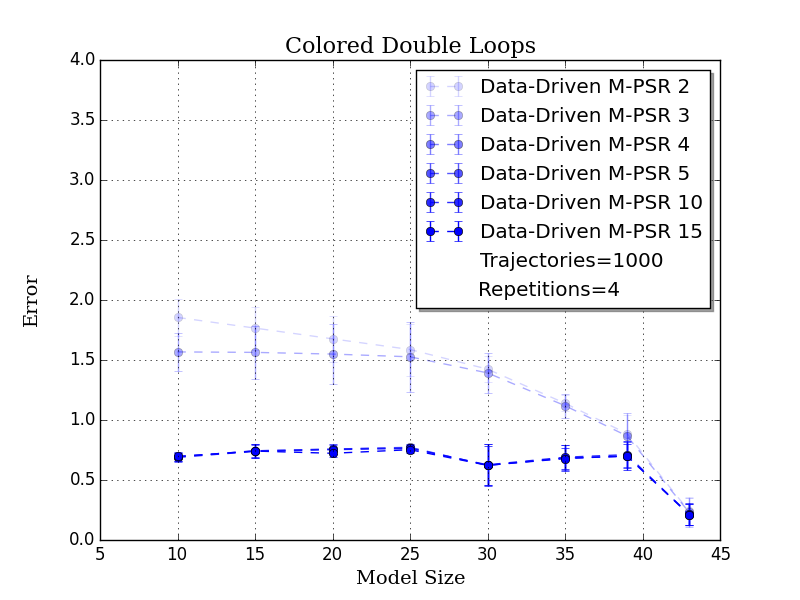
\includegraphics[width=60mm]{uCOREPICS/DLMO/numOpComparison.png}
\caption{Varying NumOps\label{fig-colnumops}}
\end{figure}
